\documentclass[11pt,letterpaper]{article}
\usepackage[top=1.00in, bottom=1.0in, left=1in, right=1.25in]{geometry}
\usepackage{graphicx}
\usepackage{latexsym,amssymb,epsf}
\usepackage{epstopdf}

\usepackage{sectsty,setspace,natbib}
\usepackage{float}
\usepackage{latexsym}
\usepackage{epsfig}
\usepackage{graphicx}
\usepackage{amsmath}
\usepackage{array}
\usepackage{lineno}
\usepackage{gensymb}
\usepackage{xr-hyper}
\externaldocument{phencc_supp}
% \usepackage{hyperref}

\usepackage{framed}

\linespread{1.1} % was 1.66 for double-spaced 
% \raggedright
\setlength{\parindent}{0.5in}
\pagestyle{empty}

\parskip=5pt
\pagenumbering{arabic}
\pagestyle{plain}
\setlength\parindent{0pt}

\begin{document}
\begin{flushright}
Version dated: \today
\end{flushright}
\bigskip
\noindent Running title: Environmental tracking 
% put in your own RH (running head)
\bigskip
\medskip
\begin{center}
% Insert your title:
\noindent{\Large {\bf How environmental tracking shapes communities in \\ stationary \& non-stationary systems}}\\
% Other titles: `Environmental tracking: It's more complicated than you think' (we hope) 
% or `Environmental tracking: Is it naive? Or, are we just naive?'
\bigskip
\noindent {\normalsize
E. M. Wolkovich$^{1}$ \& M. J. Donahue$^{2}$ }\\
\noindent {\small \it
$^1$ Forest \& Conservation Sciences, Faculty of Forestry, University of British Columbia, 2424 Main Mall, Vancouver, BC V6T 1Z4 (e.wolkovich@ubc.ca)\\
$^2$ Hawaii Institute of Marine Biology, University of Hawai`i at M\= anoa, K\=an`eohe, HI 96744 (donahuem@hawaii.edu)}\\
\medskip
\end{center}
\noindent{\bf Corresponding author:} see$^{1}$ above; Ph: 604.827.5246 (no fax).\\

\noindent \emph{Authorship statement:} EMW and MJD both conceived of the paper, performed modeling work and edited the paper, EMW additionally wrote the paper and did the literature review, while MJD additionally wrote the supplementary information on the model.  \\
\noindent \emph{Data statement:} Review, so no new primary data, but data from a comprehensive literature review will be archived in an appropriate public repository and the data DOI will be included at the end of the article. \\
\noindent \emph{Keywords:} community assembly, global change, climate change, phenology, environmental variability\\
\noindent \emph{Article type:} Reviews and Syntheses\\
\noindent \emph{Article information:} Abstract: 196 words; Main text: 5830; Figures: 4; Boxes: 3 (text in Box 1: 690; Box 2: 385; Box 3: 264); 93 references
% main text words (5500 without in-text refs approximately) ... boxes can be a max of 800 words 
\newpage
% \linenumbers % If you want to add need to add \begin{linenomath} and \end{linenomath} around all eqns (and check they still show up)

\begin{abstract} 
% FIXME
[NEED TO FIX ABSTRACT...] Climate change is reshaping the environments of all species. Predicting how communities will shift in response requires understanding the mechanisms that govern how communities assemble, and how these mechanisms will shift with warming. Growing empirical evidence suggests that environmental tracking---how much an organism can shift the timing of key life history events in response to the environment---is linked to species performance and is a structuring force in communities today.  Here, we review current knowledge on temporal environmental tracking both in empirical data and through the lens of community ecology theory. We focus on how climate change has altered the start of the growing season, examine the available evidence that tracking may trade-off with other traits, and provide an initial test of how well basic theory supports the paradigm that climate change should favor environmental tracking.  We show how trade-offs that promote coexistence in stationary environments break down in non-stationary environments and may shift the fundamental mechanisms that structure ecological communities. Finally, we consider how the reality that climate change has widespread effects beyond mean temperature, including shifts in growing season length, variability, and in extreme events, may complicate simple predictions of winners and losers. 

\end{abstract}

\newpage
\section{Main text}
Anthropogenic climate change is causing widespread changes in species distributions, with many species shifting in both time and space \citep{IPCC:2014sm}. Reports often focus on species shifting to higher elevations and poleward \citep{Chen2011} and/or shifting their recurring life history events (phenology) earlier as climate warms \citep{Wolkovich:2012n,cohen2018}. Across species, however, there is high variability. A large proportion of species are not shifting at all \citep{Cook:2012pnas}, which has raised concerns about whether these species may be more vulnerable to population declines with continued warming. Such concerns come in part from increasing research that links how well species track climate change---especially through temporal shifts---to shifts in biomass, growth and other metrics related to performance \citep{Cleland:2012}. Tracking may then be a major component to understanding and predicting the indirect effects of climate change, including population declines, with cascading effects on community and ecosystem structure.

How well a species tracks the environment through its phenology has repeatedly been linked to other species' responses to climate change. Species that phenologically track warming perform better in field warming experiments \citep{Cleland:2012}, and exotic plant species appear to gain a foothold in warming environments by phenologically tracking climate change \citep{Willis:2010al}. Simple community ecology theory supports these findings, suggesting that a warming climate should open up new temporal niche space and favor species that can exploit that space \citep{gotelli1996,wolkovich:2010fee,Zettlemoyer2019}. Thus, a shift toward earlier spring should favor earlier species, especially those that can environmentally track ever-earlier seasons. This hypothesis has gained significant traction in the ecological literature focused on global change \citep[e.g.,][]{Cleland:2012,Zettlemoyer2019}; however, there has been comparatively little work examining how tracking fits within fundamental ecological models, especially those of community assembly and coexistence. % \citep{Cleland:2012,ramula2015}

Current or `modern' coexistence theory is based strongly on understanding how variable environments may promote coexistence---providing one way to study how communities may be shaped by a temporally varying environment and how tracking may allow a species to take advantage of that variability. Most theory, however, is based on the assumption of stationarity: though the environment is variable, its underlying distribution is unchanged across time \citep[i.e., constant mean and variance,][]{barabas2018}. This assumption is common not just to coexistence theory, but to much of the theory that underlies ecology, evolution, and myriad other research fields \citep[e.g.,][]{Milly:2008yu,nosenko2013}. 

Climate change upends the assumption of stationarity. By causing increases in temperature, larger pulses of precipitation, increased drought, and more storms \citep{ipcc2013}, climate change has fundamentally shifted major attributes of the environment from stationary to non-stationary regimes. This transition is reshaping ecological systems, and, while new work has aimed to adapt coexistence theory to non-stationary environments \citep{chessonnonstat}, little work has examined what such a transition may mean for communities and the species within them.  % Importantly, models based on the theory can help highlight which species `traits,' including those related to how species are matched to and respond to the environment, are favored under different environmental regimes.

% FIXME
Here, we review current knowledge on temporal environmental tracking both in empirical data and through the lens of basic community ecology theory. We begin with a review of environmental variability in stationary and non-stationary environments as well as current coexistence theory for variable environments, then provide an initial test of how well basic theory supports the current paradigm that climate change should favor species with environmental tracking. Finally, we provide a framework using existing ecological theory to understand how tracking in stationary and non-stationary systems may shape communities, and thus help predict the community consequences of climate change. 

\subsection{Defining environmental tracking}
% Environmental variability means many species should benefit from tracking their environment. We focus here on environmental tracking through time (often referred to below as `tracking') rather than through space because of its well-established links to individual-level physiology, yielding a more robust understanding of what environmental cues determine tracking \citep{chuineJTB,Chew:2012pd}, and because it has been repeatedly linked to performance and other fitness-related metrics. Temporal environmental cues, however, are often linked to species' ranges \citep{Morin:2008vp,arabid2011}, thus we expect much of this work could extend to environmental tracking through space. 
% Definition of tracking: correlation between a recurring biological event and something else in its environment
We define environmental tracking as the timing of life history events in response to proximate abiotic environmental cues (CITE CHMURA, e.g., daylength, temperature). The first part of this definition focuses on the timing of life history events (phenology). While we may view some events as simple on/off switches, they are almost always defined by investment decisions as part of a continuous developmental process (CITEINOUYE). Thus, we argue these events are best considered as the outcome of a two-part sequential decision process that is repeatedly evaluated over time. At each temporal unit, an event can either happen or not (step 1) and, if it happens, there is a secondary decision regarding the size of the event (step 2). This decision process is generally applied at the level of the individual (but it could potentially apply at lower levels, for example buds on a branch, or potentially higher levels). Across time, it produces an event's distribution. After starting, many events are entrained to continue based on the underlying physiological process: for example, laying eggs within one clutch (in this example, the decision is whether to lay eggs or not and then how many to lay at each temporal unit, such as per day or hour) or flowering each growing season (in this example, the decision is whether to flower or not and then how many flowers to burst during each temporal unit, such as per day or hour). In such cases, first events at the individual-level are somewhat unique from the rest of the event's distribution. [MEGAN: Can we cite Mangel dynamic state variable models here?]. In all cases, these individual-distributions scale up to the population (or pseudo-population) level estimates of these events generally used by researchers (CITEINOUYE for an excellent discussion of the outcomes of this scaling).

Considering life history events that define part of environmental tracking as a two-part process highlights that tracking is ultimately shaped by resources that species need to grow and reproduce. This is perhaps best recognized in the literature on trophic synchrony where focus is often on how well consumers' environmental tracking matches to the seasonal distributions of their prey \citep{deacy2018,kharouba2018}. For example, decades of work has studied how birds (e.g., \emph{Parus major}) time their peak food demands---during their nesting season---to maximum prey (caterpillar) abundance \citep[e.g.,][]{charm2008}. Failure of environmental tracking to match prey year-to-year or over time with long-term warming has been well tied to individual-level fitness consequences in some systems \citep{charm2008}, but not all \citep{visser2006}. Environmental tracking in plants and other lower trophic levels is also about resources. Alpine plant species that emerge in step with snowmelt or temperature are likely responding, at least in part, to light resources for photosynthesis. Light equally appears critical to the sequence of phenology in many temperate forests: with lower-canopy species, and younger (shorter) individuals of higher-canopy species, routinely risking frost damage to leaf out before the canopy closes and access to light becomes severely reduced \citep{Vitasse2013,heberling2019}. In both temperate as well as alpine systems, however, access to critical belowground resources also occurs in the spring---both for available water and for nutrients released with the turnover of seasonal microbial communities \citep{Zak:1990ar,edwards2010N}. Thus, plants' spring phenology in many systems is about careful tracking to optimally compete for nitrogen and other soil resources. As in higher trophic level systems, research has linked how well plants track to performance, with species that track warming tending to grow larger and/or produce more offspring \citep{Cleland:2012}.

These ultimate controllers on tracking are filtered through the abiotic environmental cues species use to time events.Many (or potentially all) species use abiotic cues to trigger major phenological events. These cues in turn result in different rates of tracking. At one extreme, some cues yield a fixed timing, resulting in no tracking over time. A common example of a fixed cue is photoperiod, which results in event timing that is constant across years (but variable across space, allowing---for example, later timings poleward for spring events) and appears widespread for some insect emergence and for fall senescence of many trees \citep{Denlinger2017,lechowiczbook2002}. Fixed timings are perhaps the simplest option and may be efficient for events where there is low predictability, low variability, or low costs to being too late or early. In cases where there is a high cost to mis-timing an event across a variable environment, cues that yield more variability in timing are far more prevalent and usually rely on climate. Temperature is a widespread cue for start of season events with many organisms needing a certain thermal sum to start visible growth. Such a cue has the benefit of shifting the date of an event early or late, depending on climatic conditions, each year, but may be a poor cue in years with aberrant events (e.g., a late frost). In most systems, species must use environmental cues such as temperature to forecast the ideal date for an event---a date which is only obvious in retrospect. ...  Measuring tracking depends on many factors (see Box `What underlies variability in species tracking?'). 

 
\subsection{Interspecific variation in tracking}
% ADD  some numbers on variation in tracking ... why the variation? (1) it's hard to measure (keep this quick? Reference box?) and (2) maybe it's not always optimal to track ... boom, coexistence theory to the rescue!
Despite the clear importance of tracking for resource access, not all species appear to track their environments equally well \citep{thackeray2016}. Many plant species track spring temperatures strongly \citep[multiple meta-analyses now show plants' spring phenology on average track spring or annual temperatures 4-6 days/$\degree$C][and simple temperature models can often explain over 90\% of interannual variation in phenology]{Richardson:2006qh,Wolkovich:2012n,thackeray2016}, but other species do not \citep{Cook:2012pnas} and do not appear linked to other major climate variables \citep{thackeray2016}. Variability equally exists when examining consumers tracking their prey \citep[across diverse species tracking over time is 6.1 days/decade but ranges from zero to 15 days/decade, see][]{kharouba2018}. Such variation in tracking across taxa is driven in part by difficulties in measuring tracking (see Box `Statistical challenges in measuring tracking'). Yet other variation may be real and suggests perfect environmental tracking may either not be possible or optimal for all species. 

Within populations, life-history can help predict how much individuals should track while also balancing trade-offs within and across seasons and years. Tracking has been repeatedly linked to fitness benefits \citep[e.g.,][]{farzan2018,deacy2018}. Such benefits usually break down into avoiding tissue loss or maximizing growth and, relatedly, maximizing reproduction. For species with bounded growing seasons, much literature has reviewed how tracking is a multivariate equation balancing early-season access to resources and its associated risks of tissue loss, with later season tracking of resources for reproduction and time for offspring to mature \citep{donohue2002,Morin:2005ye,Burghardt2015}. These trade-offs should also scale up to predictions of variation in tracking across species. % Species often track the start of growing seasons to avoid substantial tissue loss, for example from frost damage in temperate plants, or start activity only when resources for growth are present, such is the case in animals coming out of hibernation in cold regions. Equally, tracking of resources throughout a season is linked to the timing of reproduction for many species and, for iteroparous species, decisions on how much to invest each season requires estimating how likely a year is to be good for offspring.

Across species, community ecology theory makes predictions for suites of traits that may trade-off with tracking. As tracking often relates to the timing of a resource pulse, traits related to resource acquisition are likely contenders for a trade-off. Species with traits that make them poor resource competitors may need to track the environment closely to take advantage of transient periods of available resources, but will risk tissue loss to harsh environmental conditions more prevalent early in the season (e.g., frost or snow). In contrast, species with traits that make them superior resource competitors may perform well even if they track environments less closely, because their resource acquisition is not strongly constrained by competitors. Examples include under-canopy species leafing out earlier to gain access to light \citep{heberling2019} or species with shallow roots starting growth sooner in an alpine meadow system, while species with deeper roots begin growth later \citep{Zhu2016BioLetters}. In such cases, tracking is akin to a competition-colonization trade-off \citep{Amarasekare:2003tq}, where species that track well gain priority access to resources and, thus, may co-exist with superior competitors. Research to date supports this, with several studies linking higher tracking to traits associated with being poor competitors \citep{Dorji2013,lasky2016,Zhu2016BioLetters}. Further, many studies have found a correlation between higher tracking and `earlyness' each season, which has been linked to resource acquisition traits associated with lower competitive abilities \citep[][see Box `Trait trade-offs with tracking']{wolkovich2014aob}. 

These trade-offs with tracking, predicted by basic ecological theory and tentatively supported by growing empirical work, would have fundamental consequences for community assembly, especially with climate change. Applying ecological theory to current environments, however, is difficult because most theory has been developed for stationary systems, which are mathematically more tractable, but can sometimes be extended to non-stationary systems \citep{chessonnonstat}. Almost no community assembly research, however, has examined the consequences of shifting from a stationary to non-stationary environment. % Yet this transition is exactly what anthropogenic climate change has imposed on systems around the globe, making our understanding of how environmental tracking fits within community assembly theory critical. 
% .... that would have fundamental consequences for community assembly---at least in stationary systems. In non-stationary systems, theory is less developed for how tracking may trade-off with other traits (CITECHESSON), and even less theory predicts the consequences if the environment shifts from stationary to non-stationary

% How to explain warming experiments where researchers have identified links between performance and tracking, 
% links between tracking and performance in warming experiments could potentially wash out over longer timescales (fitness not measured over long enough timescales to consider diverse species life history strategies)

% consider cost of static timing (cheap) versus tracking (potentially costly)
% Variation in tracking may also be predicted based on historical effects ... change in environment (species track old environment)
These include the costs to the organism of having a cue (or system of cues) to the environment (e.g., the machinery of monitoring temperature or daylength), the benefits of a cue (for example, how much tissue is saved by avoiding a coldsnap) and any constraints, such as cues that cannot be developed or evolutionary history making some cues more likely. 


%  All these approaches  are focused on the proximate level---what environmental cues underlie tracking---at the ultimate level tracking is shaped by what resources species need to grow and reproduce. 
% The complex cueing mechanisms that drive environmental tracking interact with and shape patterns of resource acquisition and expenditure.”


\subsection{Environmental variability \& change}

Decades of ecological research highlight how temporally variable environments shape species and their communities at multiple scales \citep{Sale:1977oq,Chesson:1997dz}.  In seasonal landscapes, the environment limits periods for growth each year (e.g., by temperature or drought); within-year variability in the environment (e.g., daily, hourly or finer resolution temperatures or rainfall amounts) compounds into inter-annual variability that shapes the distribution of the start and end of growing seasons. For long stretches of history this variability has been stationary; that is, the underlying probability distribution that describes the start (or end) of the season (e.g., the date of the last major frost) does not change, even though the date may be dramatically different from one year to the  next. % The shape of this underlying distribution varies across systems and in how it is measured---for example, the total amount of rainfall across years in semi-arid systems is often highly skewed (rare high rainfall years, with many more below-average rainfall years) compared to the more normal (Gaussian) distribution of the thermal sum of temperate growing seasons. 
% In seasonal landscapes, periods for growth each year are limited (e.g., by temperature or drought), and species must manage within-year variability by timing when to grow and when to reproduce \citep{donohue2002}. 

In other time periods, variability has been non-stationary in one or multiple dimensions. For example, climate in the northern hemisphere includes long warming and then cooling periods (i.e., increasing then decreasing means of the probability distribution) at the start of the Holocene, when the earth was coming out of the last glacial maximum. Anthropogenic climate change (henceforth, referred to simply as `climate change') is a similar non-stationary process, with warming evident around the globe and knock-on effects for other climate metrics, such as heat extremes and the size of precipitation events. While only several decades ago, ecology was focused strongly on stochasticity in stationary systems \citep[e.g.,][]{Ripa1996,Kaitala1997}, climate change has shifted the focus to understanding stochasticity in a non-stationary framework \citep[e.g.,][]{cazwavelets,ehrlen2016,legault2019}.

Understanding non-stationarity in ecological systems requires first identifying which aspects of the environment have shifted---and how they have shifted with respect to one another---as the underlying  distributions transition from stationary to non-stationary (Fig. \ref{fig:climdat}). For example, with climate change, warming has increased mean temperatures over time, with minimum temperatures generally increasing more than maximum---this results in an underlying distribution for daily temperature where the mean is increasing through time while the within-day variance is decreasing \citep{ipcc2013,screen2014}. 





\subsection{The role of the environment in coexistence} % or Coexistence theory \& environmental tracking 
Recent advances in coexistence models, sometimes called `modern coexistence theory,' recognize that both mechanisms independent of fluctuations in the environment (e.g., R* and other classical niche differences) and mechanisms dependent on fluctuations in the environment (relative non-linearity and storage effect) can drive coexistence \citep{Chesson:1997dz,Chesson:2000vd}. Models under this paradigm are thus often composed of parameters that the describe the environment and the species within it. Parameters related to species must always include mechanisms for growth, death, interactions with other species, and generally a bet-hedging strategy for survival across years (e.g., a seedbank or other long-lived lifestage)---though exactly how these are defined varies across models.
% Models under this paradigm are thus often composed of parameters that the describe the environment and the species within it (Megan--suggest CITES [working on it])

How the environment is defined in most coexistence models falls into two broad categories. In some models the environment is expressed as variation in parameters related to species (e.g., in some lottery models the environment appears, effectively, as variation in birth and death rates). In other models, the environment is more specifically defined. For example, many seed germination models define an environment that begins with a resource pulse each year. Building a changing environment into models thus may require knowing how environmental shifts filter through to species-level parameters \citep{Tuljapurkar2009} or---perhaps more simply---how the environment is changing. % In the aforementioned seed germination models for example, many systems may be experiencing shifts in the size or variability of the resource pulse. 
%[I like how this is framed, but  what is coming to mind for me is the idea of the environment coming into models as "species response to the environment", and not the environment itself.  This is the lottery model example you provide.  In some ways, our model takes both approaches - the germination function is more a a species response to envt - it essentially defines how a species responds to a particular tauP - but the resource level is, itself, the level of thresource in the system,. So our between year effects are species-response to envt and within year are more actual envt.  I'm not sure this is a helpful comment...]
% \citep{Davison2010,morris2008,Tuljapurkar2009}
% Lottery model: Birth and death rates vary ... collapses to single ratio (that's the environment) ... many general models are like this, they just vary a parameter and assume it is varying in response to the environment. Whatever parameter you allow to vary is how you allow the environment to filter through. (Side note: Tulja Purqur may have worked on how environment filters through to many species parameters in the model.)

These models, which underlie much of current community ecology research \citep{Mayfield:2010fe,barabas2018,ellner2019}, allow tests of basic predictions of how tracking may shape communities.


\subsubsection{Future research in environmental tracking \& non-stationary systems}
As we have reviewed, growing empirical research highlights that environmental tracking is linked to species performance and, thus, may be critical to understanding the forces that assemble communities and determine species persistence---especially as anthropogenic climate change is reshaping the environment of all species. Current models of coexistence are clearly primed for understanding how a variable environment can shape the formation and persistence of communities. Moving forward, we need more focus on understanding the attributes of an environment shaped strongly by humans, and, thus, what advances in theory may be most useful for making predictions in the Anthopocene. To this aim, we review several major questions that we believe could most rapidly unite empirical and theoretical research in environmental tracking to advance the field.\\ % Including non-stationarity in ecological theory is non-trivial \citep{chessonnonstat,legault2019}, but is the current environment in which all observational ecology occurs.

\emph{How is the environment changing?} \\ % Which abiotic aspects of the environment are changing? How are they shifting?

Climate change has shifted the environment of all species, often in multivariate ways (Fig. \ref{fig:climdat}). Most systems are seeing increases in mean temperatures, which can rapidly impact the metabolism and activity periods of many species \citep{Monson:2006vt,IPCC:2014sm}. This warming is also altering many other attributes of the climate system, including precipitation regimes \citep{Diffenbaugh2015}, and cloud cover \citep{hofer2017}, which can all further influence species via altering environmental cues. 

While we focused on one major shift in the climate system (earlier growing seasons), much more research is needed to understand how multivariate environmental shifts may alter these predictions. Ecologists can guide these efforts by identifying environmental shifts that are often linked (e.g., warming temperatures may drive earlier seasons and higher evaporative loss of some resources such as water). Researchers can also aim to more consistently and fully characterize the environmental distributions of their systems that appear to most drive species performance and interactions: the environment of the years of study should be clearly reported and compared against long-term and recent climate for each system.\\

\emph{What major traits trade-off with tracking?} \\

Basic theory requires that environmental tracking must trade-off with other traits to allow multi-species communities. Yet to date empirical work has mainly documented tracking, linked it to performance, or focused on how it varies between native and non-native species \citep{Willis:2010al,wolkovichAmBot2013,Zettlemoyer2019}. Such work lays the groundwork that environmental tracking is important, but future empirical research should address how this trait co-occurs with other traits. Research has highlighted some traits that co-vary with tracking \citep[e.g.,][]{kharouba2014,lasky2016,Zhu2016BioLetters}, but to tie this empirical work to models requires more research on traits that link clearly to theory, and a fuller understanding of how tracking and other traits jointly contribute to performance under varying environments. Traits that link to resource competition, as we focus on here \citep[as others have as well, see][]{volkerass}, may be especially fruitful for greater research, but should not be the only ones considered. For example, traits related to predator tolerance or avoidance may also play a role, but have been effectively unstudied.  As empirical research in this area grows, models can aid progress in understanding the outcomes of these trade-offs for community assembly.\\ 

\emph{How do shifts to non-stationary environments re-shape the relative influence of stabilizing versus equalizing mechanisms?} \\

Our simple models showed that as environments shift from stationarity to non-stationarity, species that co-occur via equalizing mechanisms can persist longer. While this is a rather obvious outcome---as equalized species will be more similarly affected by environmental shifts---it has several important implications. First, it may make identifying which traits climate change promotes through stabilizing mechanisms more difficult. Second, it suggests climate change---or other factors that cause an environment to shift from stationary to non-stationary---may cause a fundamental shift away from assembly via stabilizing mechanisms. Thus understanding the prevalence of stabilizing versus equalizing mechanisms \citep[which ecology has worked on for many decades,][]{Caswell:1976np,Chesson:2000vd} becomes critical for understanding the implications of transitions to non-stationary environments. 

If equalizing mechanisms are rare in natural communities then climate change could promote species loss by fundamentally re-shaping stabilizing mechanisms. This finding, however, comes from our modeling approach here, which assumed a closed community without  dispersal or evolution. In practice, dispersal of species or individuals with traits that make them better matched to the non-stationary environment (e.g., fixed intrinsic start times that are earlier or with a suite of traits that match to the transformed trade-off axis) would lead to new communities that may persist longer or be continually re-assembled as long as the environment remains non-stationary. Indeed, this logic underlies the argument that invasive species may be superior trackers benefiting from how climate change has altered growing seasons \citep{Willis:2010al,wolkovich:2010fee}. Evolution equally could alter our findings by allowing species traits to evolve in step with environmental change. Long-term population \citep[e.g.,][]{colautti2017} and resurrection studies \citep{wilczek2014,yousey2018}, as well as field experiments \citep{colautti2017,arab2019}, have repeatedly shown species can shift to earlier flowering times, higher thermal tolerances or related genetically-controlled traits that confer higher fitness in warmer climates. Yet these studies also highlight that responses can be lagged \citep[e.g.,][]{wilczek2014}, associated with reduced population viability \citep[e.g.,][]{colautti2017}, or other factors that may constrain adaptive responses
% In practice, communities may lose species but also gain new species through dispersal, allowing communities to potentially adjust to new trade-offs as the environment shifts. In addition, evolution may allow some species to stay in communities they would otherwise have been lost from. 
% But with non-stationarity this axis is constantly shifting---so continual community change via species loss, gain and reshaped species via evolution may be the expectation, until the environment shifts back to stationarity.

\subsection{Stationarity in the future}

While most environments today are climatically non-stationary and have been for decades, the climate will return to stationarity in the future. There are many possible pathways to climatic stabilization, but almost all require first the stabilization of greenhouse gases---the subject of much policy and political debate. Once greenhouse gas emissions stabilize climate will not quickly snap back to a new stationary phase. Instead systems will slowly approach a new climatic stationarity depending on how they are effected by the earth's multiple thermal reservoirs, and, in turn, how quickly those reservoirs stabilize. The timescale of this approach is generally expected to be on the scale of centuries, but could be much longer in certain oceanic systems \citep{ipcc2013ch12}. Thus, ecologists are---and will remain for the forseeable furture---in a research area structured by climatic non-stationarity. 

As paleobiologists and evolutionary biologists often point out, climatic nonstationarity is a common part of the earth's history \citep{Jansson:2002nz}---even if stationary periods---be they cold or warm (glacial and interglacial periods)---are more common. Indeed, while much of this work has examined how species survive for millions of years given large oscillations in climate \citep{provan2008}, the periods that provide the most dramatic community reshuffling are periods shifting from stationary to non-stationary climate regimes \citep{vrba1980,vrba1985}. Such stories of the past are now fundamentally happening today, and ecology is challenged to understand how transitions between stationary and non-stationary environments are reshaping the species and communities we have today and will in our warmer future. 

\section{Acknowledgments}
We thank I. Breckheimer, D. Buonaiuto, E. Cleland, J. Davies and G. Legault for helpful comments that improved the manuscript and the NSERC Discovery Award (RGPIN-05038 to EMW) and Canada Research Chair in Temporal Ecology (EMW) programs that provided funding. 

% Chapter 12 of IPCC WG1 "Long-term Climate Change: Projections, commitments and irreversibility" (Section 12.5: Climate Change Beyond 2100, Commitment, Stablizition and Irreversibility)

% Note to self: environmental tracking seems used by spatial folks ...
   % https://www.nature.com/articles/srep36265
% But! The temporal autocorrelation folks use it too ... this is mainly one-site population work I think and pretty damn similar to our use!
   % https://royalsocietypublishing.org/doi/10.1098/rspb.2011.0487 (2011)
   % https://link.springer.com/article/10.1007/s12080-015-0276-6 (2016)
   % https://besjournals.onlinelibrary.wiley.com/doi/full/10.1111/1365-2745.12077 (2013) 
% And this annual review has a whole section (no definition though that I saw):
   % https://www.annualreviews.org/doi/full/10.1146/annurev.ecolsys.35.120202.110110 ... about fossil 'The principal cause for these patterns appears to be species-, and perhaps clade-level, environmental fidelity that results in long-term tracking of physical conditions. ... biotas do appear to track climates, but such tracking is certainly influenced by geographic and physicochemical barriers' 
% So I say it is all the same thing! And we focus here on the temporal aspect .... give nod to space at the end of ms maybe?

\section{Box: What underlies variability in species tracking?}
Much recent research in phenological tracking has focused on variability across species \citep[e.g.,][]{Willis:2008bf,Cook:2012pnas,bolmgren2013,CaraDonna2014}, with growing work highlighting that some species do not appear to track climate closely. Indeed, theory predicts some species, for some events, should not track the environment, but identifying non-trackers is difficult in most systems. % Progress in understanding how tracking may structure current and future communities requires identifying variation in tracking across species, but this task is difficult in most systems.

We argue three majors classes of reasons underlie species that do not appear to track climate: (1) species do not track, (2) lack of firm biological understanding of the cues that underlie tracking, and (3) statistical artifacts that make it difficult to measure tracking robustly (see Box `Statistical challenges in measuring tracking'). In some cases, species may be best served to not track; this includes species in highly variable environments or which otherwise face high uncertainty in when to time investment decisions. In such cases, species should gain a substantial benefit from bet-hedging or employing other approaches that spread out risk given uncertainty \citep{Venable:2007os,donald2013}. Additionally, evolutionary limitations may prevent tracking: species may not be able to closely measure relevant environmental cues \citep{arnold1992,Singer:2010eb}, gene flow from other environments may continually push a population away from its local optimum \citep{lenormand2002}, or there may be unavoidable trade-offs \citep{levins1968} with tracking.  Growing evidence suggests a potential fundamental trade-off where early species track and possess a suite of traits to related to faster growth and shorter lifespans, while later species track less and possess traits related to slower growth and longer lifespans---these later species may bet-hedge more given their longer investment window. This, however, could equally be an artifact where early species use simpler cues, and, thus, their tracking is measured more accurately given current methods. 
% Predictability depends on the timescale of interest, which is related to a species' generation time \citep[which itself should be shaped by an environment and its predictability,][]{Davison2010,morris2008}. 

Accurately measuring environmental tracking depends on the temporal scale of the question (e.g., intra-annual versus inter-annual versus decadal), and how well researchers understand a species' underlying physiology and ecology. Tracking is often measured simply by the relationship between the dates of the phenological event and a simple abiotic metric, such as mean monthly temperature (with variation in temperature derived from multiple periods of observation or induced through experiments). Simple environmental metrics, however, are almost always proxies for a more complicated underlying physiology where simple cues---such as warm temperatures---can be modified by other cues, such as photoperiod, drought or light spectra \citep{Bagnall1993,Stinchcombe:2004ec}. Indeed, multiple studies have shown how simple correlations between phenological events and environmental variables can mask complicated relationships \citep{Cook:2012pnas,tansey2017}. Most well-studied species have multiple cues to time critical biological events \citep{chuinearees}. These additional cues almost always appear adapted to handle unusual---though not completely uncommon---years when the simple cue alone would fail (that is, would trigger growth, reproduction or another life history event at a suboptimal time). 

Modeling this multi-cue complexity well is inherently difficult \citep{chuine2016}, especially since one cue may dominate in many conditions. For example, woody plant leafout responds strongly to warm spring temperatures, but also to cool winter temperatures to prevent leafout in mid-winter warm snaps that occur long before the last frost. Often this cool-temperature effect may be masked by sufficiently cold conditions. With warming, however, this additional trigger---which appears to vary by site, species and even inter-annual conditions \citep{dennis2003}---may become critical. In some semi-arid systems, species time growth to pulses of rain, but only when those rain events occur with cooler temperatures that indicate the start of the rainy season, and not a rare summer rainfall event in the middle of months of drought \citep{Wainwright:2012tw,wainwright2013}. Thus, despite the apparent efficacy of many current phenological models, many models may fail spectacularly in the future as additional cues come into play \citep{chuine2016}. Tracking in species with longer generation times may be especially complicated, as species may track low frequency climate signals and make investment choices on far longer timescales than species with shorter lifespans \citep{morris2008}. 

\section{Box: Statistical challenges in measuring tracking}
Perhaps the most widespread reason for observations of species that do not track is statistical artifacts, including non-stationarity in units and unrecognized low power. All of these can be addressed given improved statistical approaches, though such approaches may (uncomfortably) highlight how uncertain many current estimates are \citep{brown2016}. Non-stationarity in units comes in many forms---estimates of mean days shifted per decade (i.e., days/decade, a common metric summarizing observed shifts in phenology over time in long-term datasets) depend strongly on the climate of the decade(s) studied, which is not consistent in many systems \citep{Ault2011,McCabe2012}. Estimates based on a relevant climate variable can sometimes ameliorate this problem, but may be equally vulnerable to non-stationarity in units. For example, processes that depend on thermal sums reported as days/$\degree$C will generally appear to decline with warming, as the thermal sum of an average day has increased in most regions with climate change. Relatedly, estimates of long-term change using simple linear regression are influenced by the climate at the start of the time-series (with greater changes seen from time-series that started in unusually cold decades, such as the 1950s for much of North America). Impacts of start-years for long-term time-series can be muted by applying change-point or hinge models \citep[e.g.,][]{kharouba2018}. 

Low power is widespread in ecology, where even `long' time-series may be far too short for robust analyses \citep{bolmgren2013,kharouba2018}. Authors should be especially cautious if they find only large effects appear significant \citep[e.g.,][]{CaraDonna2014}, which is a well-known statistical bias associated with p-values \citep{loken2017}. Additionally, effect sizes that are higher when climate variability is higher (for example, in temperate habitats temperature is highly variable in the spring and autumn compared to summer) may be more related to variation in statistical power than to biology (periods with higher variation yield greater variation in the predictor variable, and thus higher power). Mixed models can help better leverage understanding by pooling information across species, and often better capture uncertainty \citep{pearse2017}. We suggest mixed models should be used more widely alongside randomization and/or data-simulation approaches \citep[e.g.,][]{bolmgren2013,kharouba2018} to better estimate and communicate uncertainty in studies. 


\section{Box: Trait trade-offs with tracking}
% Supp figure is still not showing -- comes up with ?? in Figure reference.
Research on phenological tracking and traits has increased greatly in recent years, with a major uptick in studies after 2010 (see SI Fig. \ref{fig:papertrends}). Most papers examining tracking and other traits across species have focused on plants (20/30), followed by birds and Lepidoptera (both 4/30), plankton and aphids (both 1/30). The most studied trait was how early or late a phenophase occurred (e.g., date of flowering of start of migration for a species, termed `earlyness' by some authors), with earlier species tending to track more \citep[studies included both birds and Lepidotera,][]{Diamond:2011nx,Ishioka2013,kharouba2014,jing2016,du2017}. While this is an important link, it is vulnerable to statistical challenges (see Box `Statistical challenges in measuring tracking'). Few studies examined whether tracking correlates with resource acquisition traits; those that did generally found species with higher tracking also had traits associated with lower competitive abilities under low resources \citep[e.g., being shallower or lacking a taproot rooted][]{Dorji2013,lasky2016,Zhu2016BioLetters}. These species were often also early \citep[e.g.,][]{Dorji2013,Zhu2016BioLetters}, suggesting tracking may relate to a syndrome of traits that allow species to be rapid colonizers each season, but poor competitors for resources. Indeed, previous work has documented that species with earlier phenophases tend to have resource acquisition traits associated with lower competitive abilities \citep[e.g., they tend to be of lower height, have shallower roots, narrower diameter vessels, thinner leaves, and grow faster, reviewed in][]{wolkovich2014aob}. 
% need to add Jing2016 to "studies included both birds and Lepidotera"


\section{Model box} % 628/800 words now
To understand the role of environmental tracking by species in variable environments we use a simple model that allows within- and between-year dynamics to contribute to coexistence. As the model is akin to many commonly used seed germination models \citep{Chesson:2004eo}, we follow a similar terminology for ease; however the basic structure of our model could apply to other systems with one dominant pulse of a limiting resource each season (e.g., water from rain or snowpack), or a multivariate resource pulse that acts effectively as one resource (e.g., nitrogen and light drawn down together over the season). In this model the environment is included between-years via variable germination, and within-years the environment is explicitly included as a resource pulse at the start of the season. 

In this model, biological start time, can be considered a fixed characteristic of a species, but we adjust it to also allow species to respond to the environment dynamically through what we refer to as tracking. Here, tracking effectively moves a species intrinsic start time closer to the environmental start time in that year, resulting in a higher germination fraction (see SUPP).

In this model, species can co-occur via equalizing mechanisms, but they require stabilizing mechanisms to coexist. Species that is, cannot coexist given only variation in tracking---coexistence requires variation in another trait axis. As discussed above, theory and empirical work suggest this trade-off may involve traits related closely to resource competition. With this added variation---here we varied species' $R^*$---species can persist together as long as those species with a temporal niche advantage are also the inferior competitors (Fig. \ref{fig:alpharstar}). That is, species that can draw resources down to a lower level and are thus the superior within-season resource competitors (lower $R^*$) can persist with species with that are inferior competitors but have realized biological start times closer to the environmental start time---a finding inline with currently observed empirical trade-offs (see Box `Trait trade-offs with tracking'). These trade-offs, however, are all environmentally dependent. They hold only so long as the environment is stationary. 

We examined how trade-offs may be transformed by a non-stationary environment, by transitioning a stationary environment---in which two-species communities had persisted for 500 years---to non-stationary, via an earlier start of season (Fig. \ref {fig:concept}a; see SI for more details). By changing a fundamental niche axis (the distribution of the environment, an axis along which these communities were structured), we shifted one major part of the trade-off: the new non-stationary environment favored an earlier effective biological start time than the previous stationary environment. This, in turn, reshaped our two-species communities, which depended on this trade-off for persistence. 

While the non-stationary environment favored higher trackers (who in turn drove the extinction of species with lower tracking values from many two-species communities) some two-species communities persisted (257 out of 1698 two-species communities persisting after end of stationary, or 15.1\%, Fig. \ref{fig:alpharstar}). These two-species communities persisted because the same fundamental trade-off between biological start time and within-season competitive ability, while narrowed, was not fully lost (Fig. \ref{fig:alpharstar}). Taken together, these simple simulations show how non-stationarity can drive local species extinction and reshape the underlying assembly mechanisms of communities.

Our simulations support growing work that tracking should not be considered alone \citep{Diamond:2011nx,Dorji2013,Ishioka2013,kharouba2014,du2017}, but may be part of a larger trait syndrome. Indeed, this model trivially show that multi-species communities cannot form given only variation in the temporal niche---a trade-off is required. Our results thus support empirical work showing a trade-off where trackers are also inferior resource competitors \citep{lasky2016,Zhu2016BioLetters}---we show this must be the case for multi-species persistence; otherwise, the species best matched to the environment would drive the other extinct. Finally, our results highlight that non-stationarity may reshape the balance of equalizing versus stabilizing mechanisms (discussed further below). 

\begin{figure}[t!]
\centering
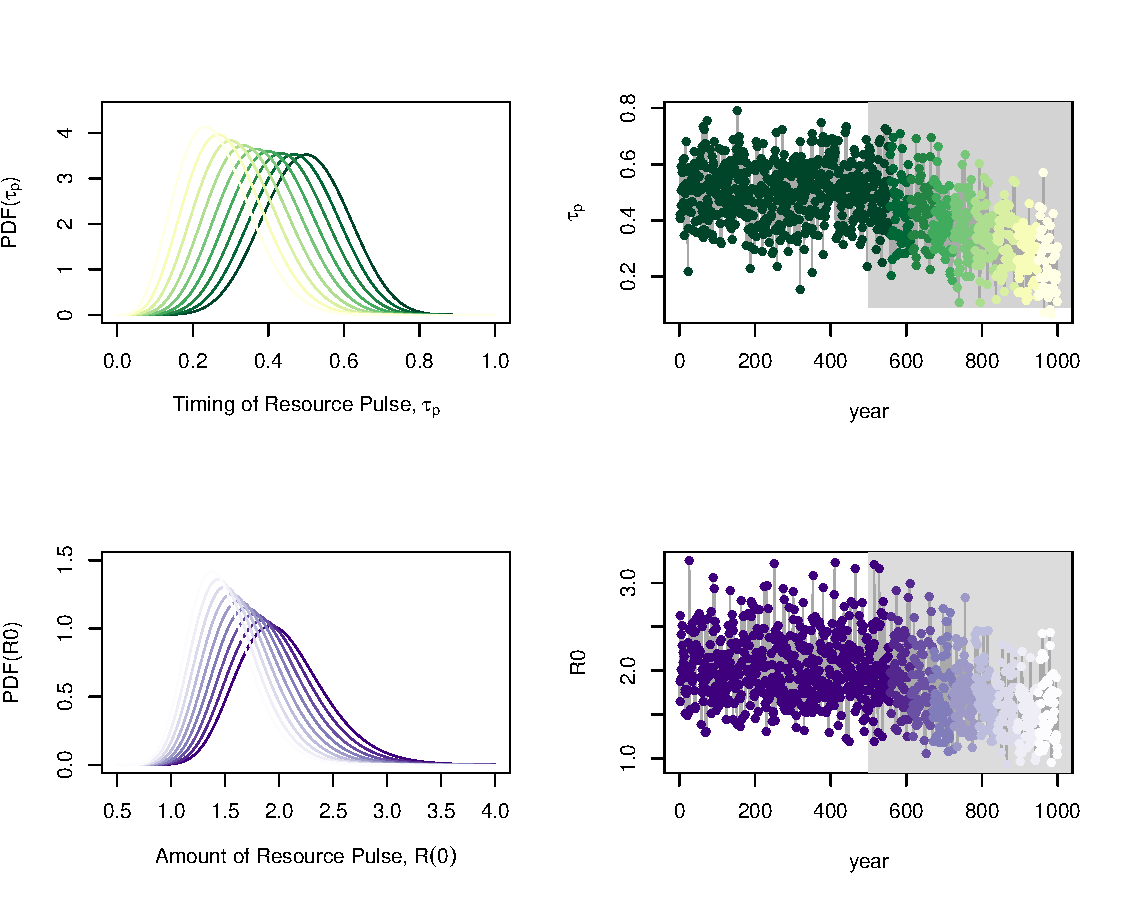
\includegraphics[width=1\textwidth]{..//..//..//R/graphs/modelruns/manuscript/modelsupp.pdf}
\caption{How the environment shifts from the stationary period to the nonstationary period. The timing of the resource pulse shifts from $\tau_{p} \sim \beta(10,10)$ for the 500 year stationary period to $\tau_{p}=\sim \beta(5,15)$ over the 500 year nonstationary period.}
\label{fig:figR0}
\end{figure}

\begin{figure}[t!]
\centering
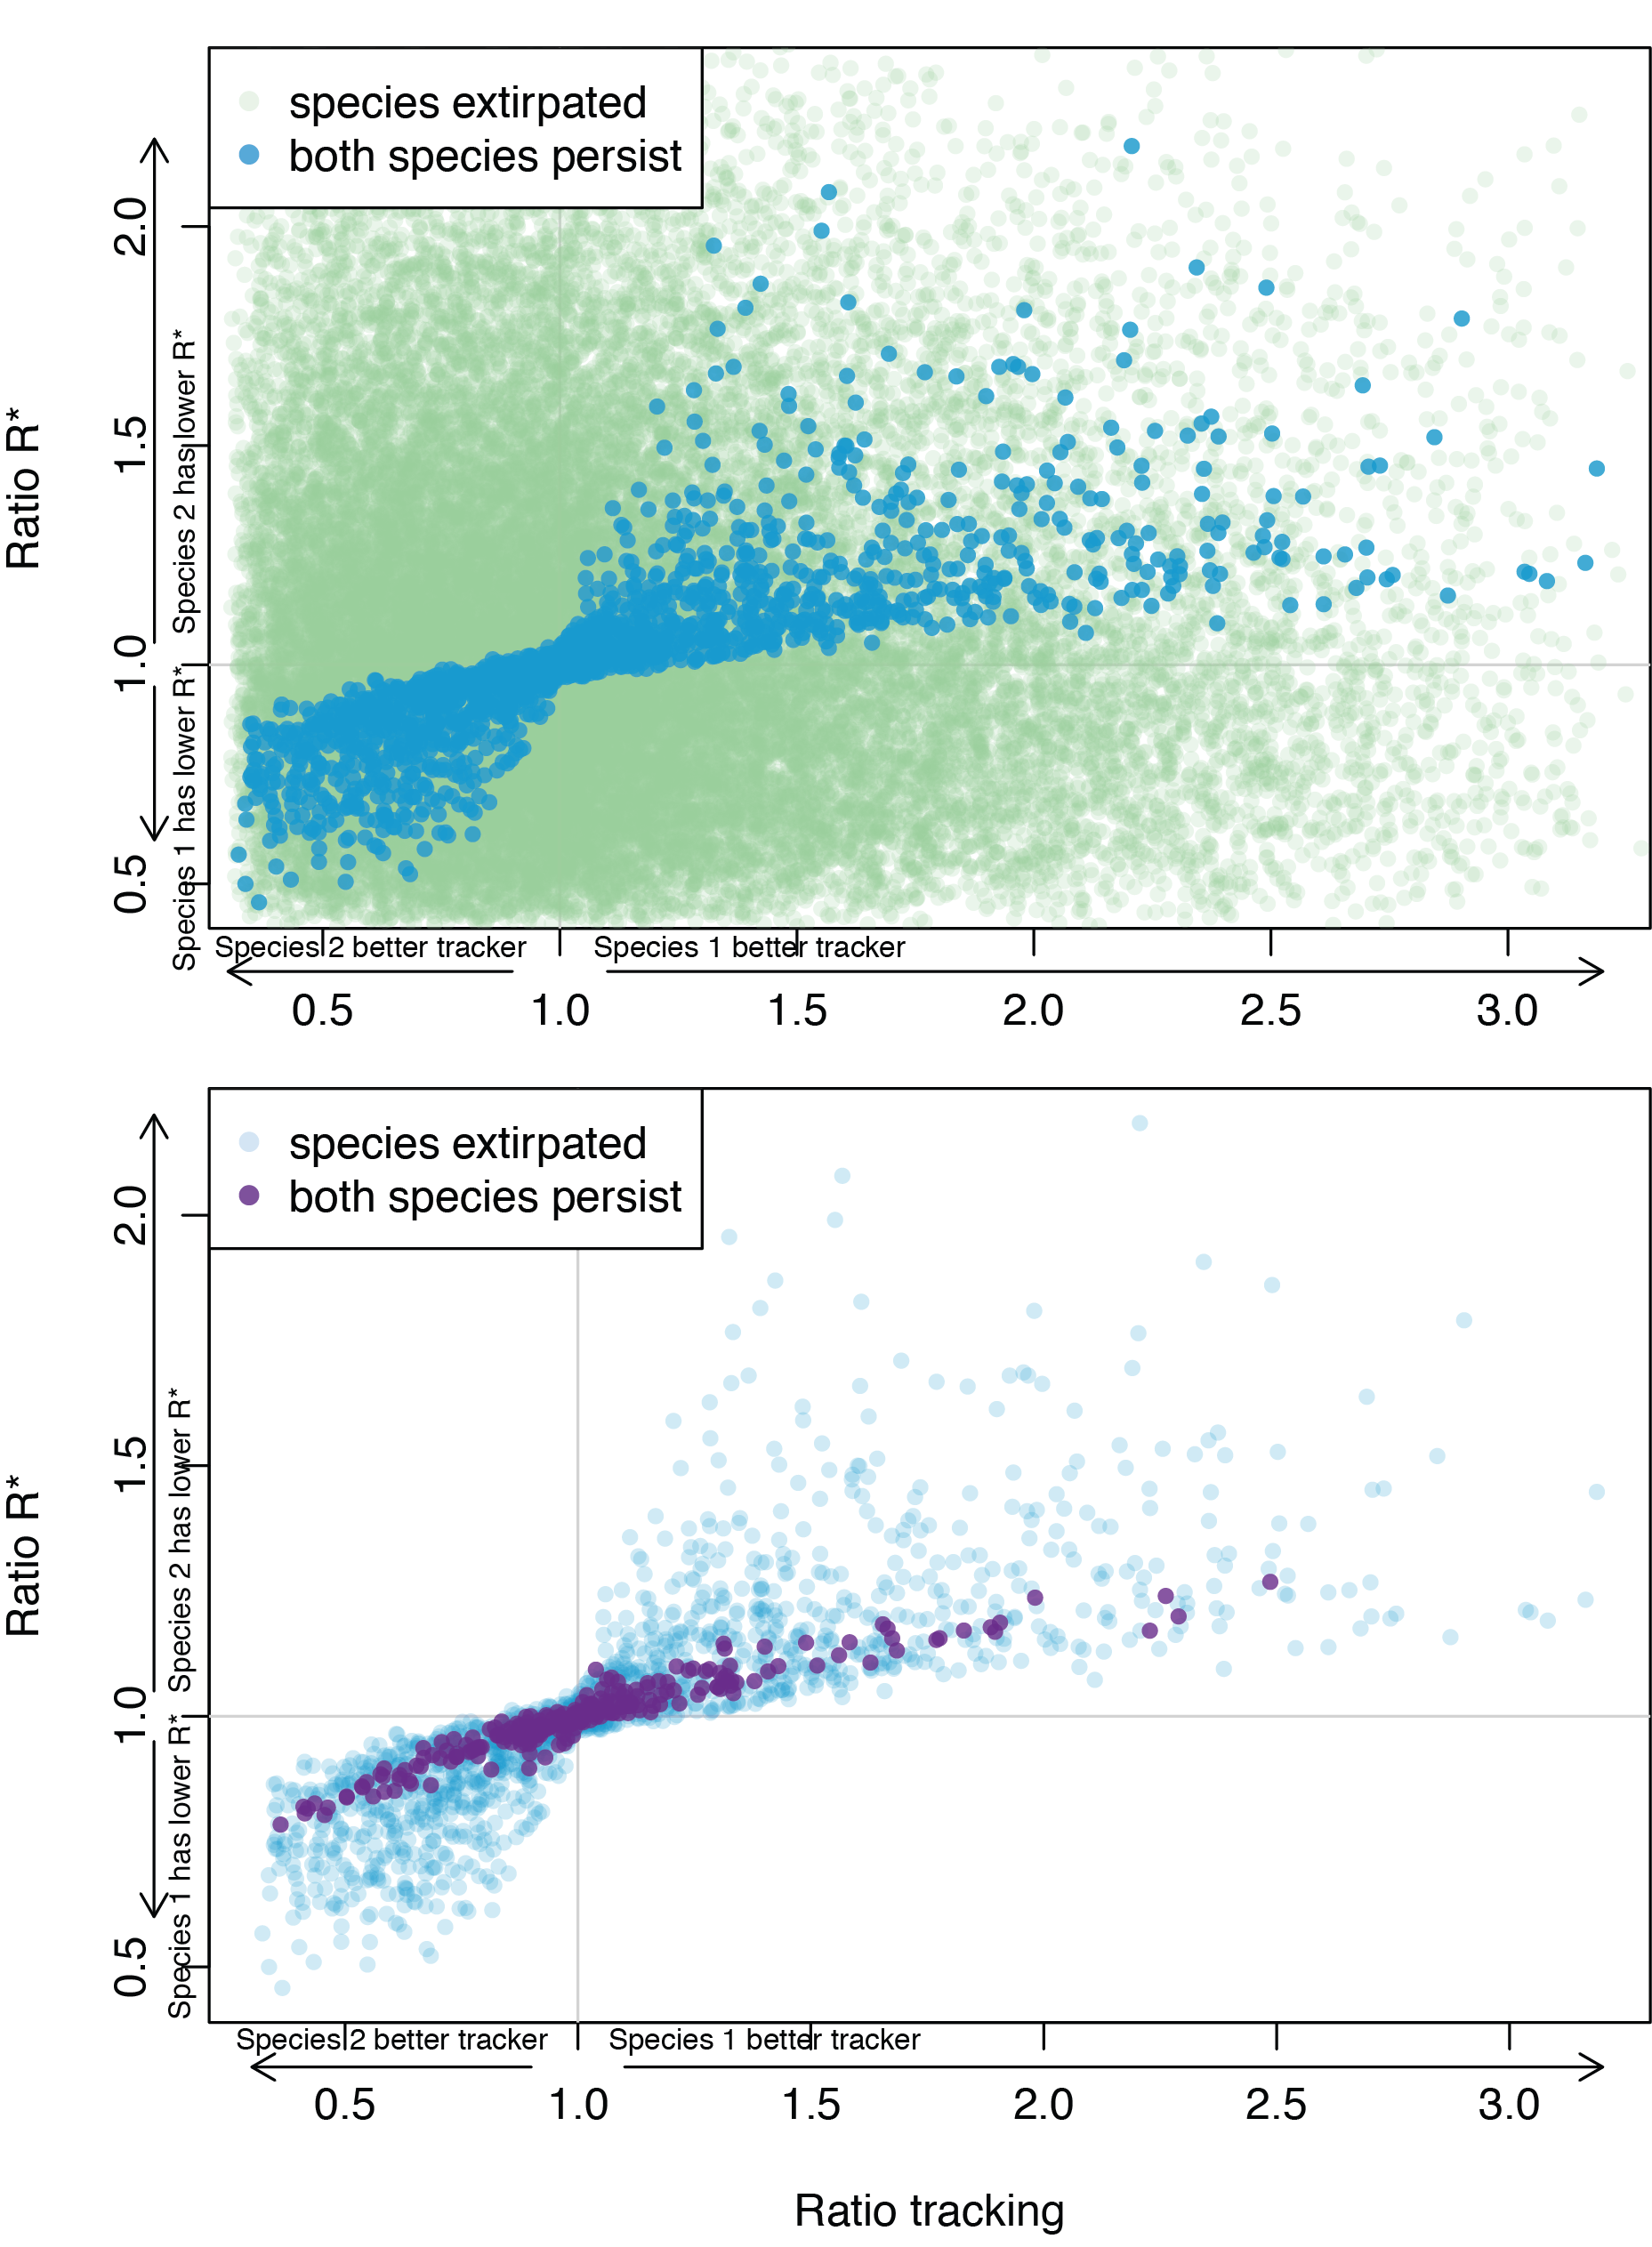
\includegraphics[width=0.8\textwidth]{..//..//..//R/graphs/modelruns/manuscript/alpharstar_2panel_adj.png}
\caption{How non-stationarity reshapes two-species communities in a simple model where tracking (X axis: species 1/species 2) trades off with $R^*$ (Y axis: species 1/species 2): each point represents one two-species community color-coded by whether both species persisted or one or more species was extirpated through 500 years of a stationary environment (top), followed by an additional 500 years of non-stationary environment (bottom), where the abiotic start of the season shifts earlier. Only two-species communities that persisted through the stationary period are shown in the bottom panel. See Fig. \ref{fig:alpharstarsupp} for an alternative version of this figure detailing one-species outcomes.}
\label{fig:alpharstar}
\end{figure}


%=======================================================================
% \section{}
%=======================================================================

%=======================================================================
%\section{Acknowledgements}
%=======================================================================



%=======================================================================
% References
%=======================================================================
\newpage
\bibliography{/Users/Lizzie/Documents/git/bibtex/LizzieMainMinimal}
\bibliographystyle{/Users/Lizzie/Documents/git/bibtex/styles/ecolett.bst}


%=======================================================================
% Tables
%=======================================================================

%\begin{center}  
%\begin{table}
%\caption{Key differences between PWR and traditional PCMs such as PGLS.}
%\begin{tabular}{ | p{4cm} | p{5.5 cm} | p{5.5 cm} |}   \hline 
%& PWR & PCMs (e.g., PGLS) \\ \hline \hline
%Major goal & Study of evolution of correlation between variables across species & Study of evolution of correlation between variables across species\\ \hline
%\emph{Assumption 1:} Nature of correlation between two or more variables & Non-stationary (changes through phylogeny in a phylogenetically conserved fashion) & Stationary (constant) throughout phylogeny (all variation is noise) \\ \hline
%\emph{Assumption 2:} Completeness of variables & Substitutes phylogeny for variables (simple or complex) not in the model that interact with variables in the model & Assumes variables in model are primary drivers of correlational relationship \\ \hline
%Inferential mode & Usually exploratory & Hypothesis testing (statistical significance)\\ \hline
%Outputs & Coefficients of regression changing through the phylogeny & p-value and single set of coefficients presumed to apply to entire phylogeny with their confidence intervals\\ \hline

%Method to avoid overfitting & Cross-validation (boot-strapped determination of optimal band-width for accurate prediciton of hold-outs) & Exact analytical model of errors and degrees of freedom\\ \hline \hline
%\end{tabular}
%\end{table}
%\end{center}

%=======================================================================
% Figures
%=======================================================================
\clearpage

\begin{figure}[t!]
\centering
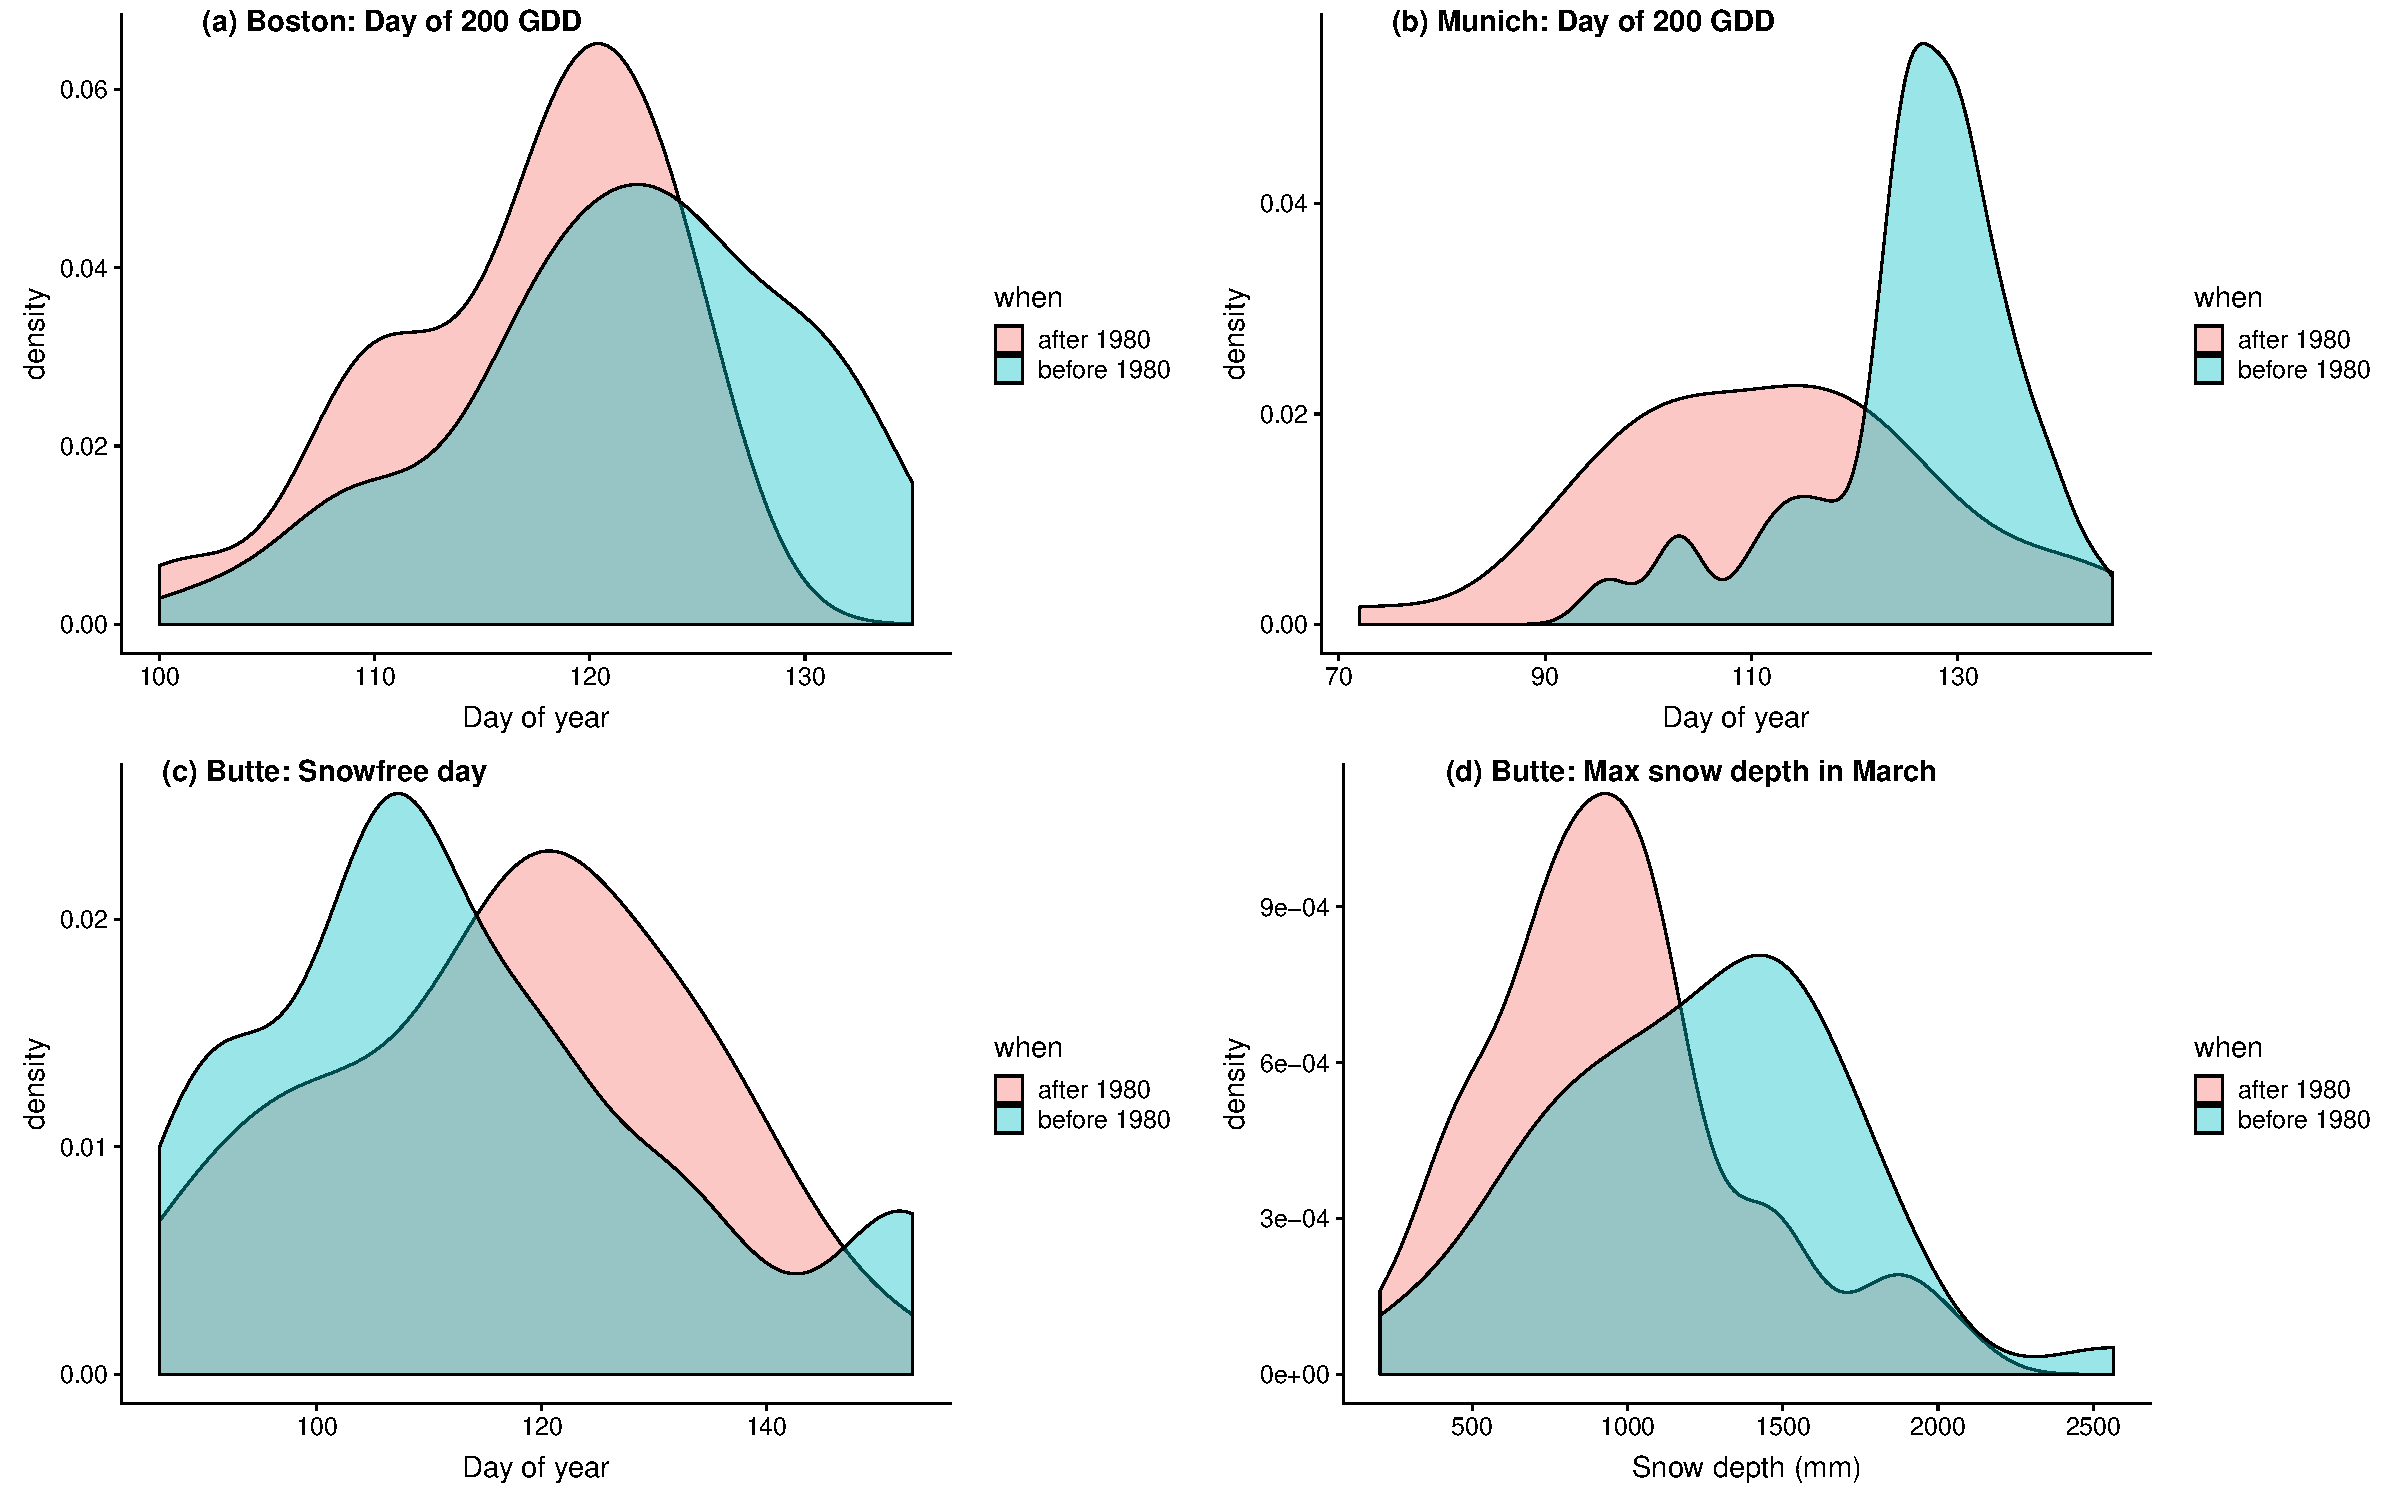
\includegraphics[width=1\textwidth]{..//..//..//R/graphs/otherdat/climdata.pdf}
\caption{Examples of non-stationarity in climate variables linked to environmental tracking: shifts before and after 1980 (a major change-point in climate for many regions) in several metrics related to the start of growing seasons (a-c) or resource pulse connected to growing season length (d). Density plots of day of 200 growing degree day units (a metric of thermal sum, here based on 0 degree base temperature using daily minima in $\degree$C) in Boston, MA, USA (a), and Munich, Germany (b), first snowfree day (followed by at least 9 snowfree days) in Crested Butte, CO, USA (c) and maximum snowdepth (mm) in March (often the month before the first snowfree day) in Crested Butte, CO, USA (d). Note that (c) and (d) are likely related, with lower snowpacks leading to an earlier first snowfree day. We selected sites that have been studied for plant phenological data and included at least 80 years of daily climate data from a Global Historical Climatology Network site; we subsetted data so that there were 40 years before and after 1980 for all sites.} %  (downloaded from \href{https://climexp.knmi.nl/})
 \label{fig:climdat}
\end{figure}





\end{document}
%%%%%%%%%%%%%%%%%%%%%%%%%%%%%%%%%%%%%%%%%%%%%%%%%%%%%%%%%%%%%%%%%%%%%%%%

\section{Figures}
\begin{enumerate}
\item Figure for ... The shape of this underlying distribution varies across systems and in how it is measured---the amount of rainfall in semi-arid systems is often highly skewed compared the thermal sum of many temperate growing season
\item With climate change, warming has increased mean temperatures over time, with minimum temperatures generally increasing mre than maximum---this results in an underlying distribution for daily temperature where the mean is both increased through time and the variance is decreasing (Munich garden? Maybe add San Dieg precip example?
\item Real-world data showing stat/non-stationarity in environment (ideally $\tau_{p}$) 
\item Real-world data showing tracking (and less tracking)
\item $\tau_{i}$ vs. R* trade-off and histogram of persisting $\tau_i$ under stat/nonstat $\tau_{p}$ environment
\item alpha vs.$\tau_i$ trade-off and histogram of persisting alpha under stat/nonstat $\tau_{p}$ environment
\item alpha vs. R* trade-off and histogram of persisting alpha under stat/nonstat $\tau_{p}$ environment
\item (Scratch this one: we're pretty sure it required a crappy $\tau_i$ to survive the initial stationary period, then be favored in second time period and we're not so sure crappy $\tau_i$ species survive the initial stationary period) time-series of one run showing years where $\tau_i$ of one species is close to $\tau_{p}$ and other years where $\tau_i$ of other species is close to $\tau_{p}$ (and show this shift under nonstat)
\item non-stationarity in $R0$ and $\tau_{p}$
\end{enumerate}


%=======================================================================
% to-do listing
%=======================================================================

\listoftodos

%=======================================================================
\section*{Other loose ends}
%=======================================================================

% Old hypothesis: Without tracking we may predict benefits to early-colonizers decline with earlier seasons. As start-date moves earlier, early folks lose benefit (assuming they tend to often go at optimum time) and you get more late folks. Late species may be less different than one another---and less responsive to environment. Early folks, effectively, become more similar to environment. 



% Old parts of intro not currently used....
Athropogenic climate change is causing widespread changes in species, with many species shifting in both time and space (CITES). Many species are shifting in ways predicted by a direct response to track climate---for example, species are shifting up in elevation and poleward as climate warms (CITES), and/or shifting earlier in their recurring life history events (phenology)(CITES). Yet, not all species are shifting as predicted by a simple climate-tracking response; species in the same community can include some that do not shift or even shift in an apparently opposing direction (e.g., delayed spring phenology with warming). \\

Understanding these variable responses of species and communities to climate shifts is a major aim of current ecology and may be explained by indirect effects. Research has already documented changes in a species performance (CITES) and community composition that appear to be---at least in part---indirect effects (CITES).  Understanding ecological responses to climate change will thus require synthesizing information on both direct effects of climate on species and indirect effects driven by responses to other species' shifts. \\ % Alongside these more direct physiological effects of climate change, however, are indirect effects.






